\subsubsection{Site Overview}\label{overview}
Si fa riferimento alla pagina: \\
\url{http://www.alexa.com/siteinfo?ax_atid=3dcecff3-eaba-4eb2-98d8-af635c113373}
\begin{figure}[ht]
\centering
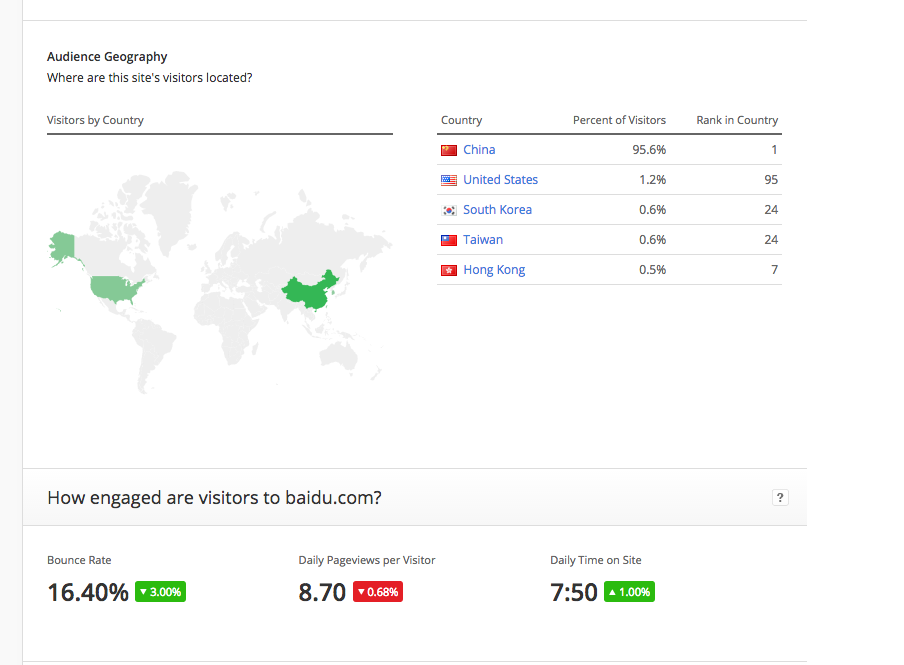
\includegraphics[scale=0.35,keepaspectratio]{{figure/4/siteOverviewSearch1}.png}
\caption{Pagina Site Overview (primo scroll) - presentazione dei risultati di ricerca}
\end{figure}
\FloatBarrier
Altri screenshot relativi alle schermate di scroll contenute in questa
pagina sono disponibili ai path:
\begin{itemize}
	\item \textit{Figure/4/siteOverview0.png}
	\item \textit{Figure/4/siteOverview2.png}
	\item \textit{Figure/4/siteOverview3.png}
	\item \textit{Figure/4/siteOverview4.png}
\end{itemize}
La pagina permette di provare alcune funzionalità ristrette del motore di 
ricerca Alexa, è così possibile farsi un'idea concreta dei vantaggi che lo strumento
può offrire. \\
Utilizzando la barra di ricerca è possibile indicare un sito web di cui 
si vogliono calcolare le metriche. \\
La prima pagina di risultati (siteOverview0.png) mostra il traffico rispetto
agli altri siti e la posizione in Alexa Rank rispetto alla nazione di punta ed al
resto del mondo. Scrollando alle pagine si possono trovare informazioni
più dettagliate (i.e. distribuzione dei visitatori per nazione, keyword 
utilizzate per trovare il sito, altri siti visitati poco prima di approdare
al sito, pagine interne più visitate, siti correlati, distribuzione dei
visitatori divisi per occupazione etc.). I contenuti sono presentati in modo
molto efficace (grafici, percentuali, classifiche in liste numerate), 
in questo caso è 
accettabile lo scrolling in quanto sono informazioni difficilmente
frazionabili anche se divisibili per 
tipologia di metrica. Si potrebbe comunque migliorare
inserendo ogni
sottosezione di scrolling in una lista verticale (ogni elemento 
identificato da un titolo) che mostri
solo il primo elemento lasciando all'utente la scelta di quale
elemento esplodere secondo le sue necessita, in questo
modo si elimina il problema dello scrolling disponendo
il contenuto in una forma più compatta e navigabile.  
Una critica che si può fare riguarda il fatto di non
sfruttare tutto lo spazio della pagina (stessa critica fatta ad Homepage),
si potrebbero espandere i contenuti (soprattutto i grafici in modo
da renderli più facilmente leggibili) allargando le 
informazioni in modo che occupino tutto lo spazio disponbile senza lasciare 
colonne vuote ai margini.\\
Risultato : \textit{7.5}